\chapter{Implementation}
This chapter deals with the implementation details of the campus app. It starts by describing the process for the collection and processing of geodata and explains how the campus map and the navigation system are derived from it. It further showcases the procedure for gathering campus-relevant data from publicly available web sources and concludes with a description of the implementation process for the user interface, which finally merges the campus map, navigation and information layers.

\label{cha:implementation}
\section{Collection of geodata and POI}
Geodata refers to all data about geographic information. In the case of this thesis, it mainly consists of coordinate points, which describe certain campus-relevant entities, such as outlines of buildings, the street network, pathways, entrances as well as boundaries of green areas and water. Except for single-point usage, multiple coordinate points can be grouped into polygons, representing the closed outline of an entity and polylines, mainly used to describe lines, streets and paths. In addition to its coordinates, geodata also describes other attributes of an entity e.g., its name, altitude, width or height. This can be used for tasks like geocoding/reverse geocoding, display of information, 3d terrain generation or general data analysis.

\subsection{Overview of needed geodata}
Geodata is the building block for map generation and routing through a street network. The following list presents an overview of the geodata needed for this implementation:

\begin{itemize}
    \item Buildings: The outlines of buildings are polygons consisting of multiple coordinate points. Additionally to that, the height of each building is needed for appropriate 3D representation.
    \item Streets: Streets are represented by polylines and are (based on their importance, size and purpose) divided into three categories, namely main roads, small roads and pathways. This separation allows the different road types to be designed and displayed independently from each other. They can therefore vary in size, style and coloring when used in the campus map.
    \item Green areas: The outlines of green areas are retrieved in the polygon format.
    \item Water: The outlines of water (especially rivers) are also retrieved in the polygon format.
    \item Entrances to TU Berlin's buildings: To successfully connect TU Berlin's buildings to its underlying street network, entrances need to be defined. A single-point representation paired with an identifier for the buildings is used.
\end{itemize}

\subsection{Collection data from OSM via Overpass Turbo API}
OpenStreetMap (OSM) is a free mapping service, that allows its users to access, edit and download its available geodata. Its main querying language is Overpass Turbo which comes with a web interface for data mining and a respective web API \cite{openstreetmap_overpass_turbo}. This querying system is used to provide a starting point for the complete set of geodata needed for this thesis. The used bounding box for retrieval is (52.49993096650543, 13.307022255971093) for the south-west and (52.52269751545147, 13.341918533901309) for the north-east corner. The following table presents the queried data over all categories together with the node count (one node usually consists of a coordinate point), the type of retrieved data and the respective query.

\begin{table}[!ht]
	\small
	\centering
	\begin{tabular}{|l|l|l|l|}
		\hline
		\textbf{Entities}       & \textbf{Type of geodata}       & \textbf{Number of queried nodes}       & \textbf{Overpass Turbo query} \\
		\hline
        Buildings               & Polygons              & 1949                          & \ref{buildings} \\
		\hline
		Main roads              & Polylines             & 2036                          & \ref{main_roads} \\
		\hline
		Small roads             & Polylines             & 2578                          & \ref{small_roads} \\
		\hline
		Pathways and sidewalks  & Polylines             & 11757                         & \ref{pathways} \\
		\hline
        Green areas             & Polygons              & 5057                          & \ref{green_areas} \\
		\hline
        Water                   & Polygons              & 1651                          & \ref{water} \\
		\hline
        Entrances               & Single points         & 1758                          & \ref{entrances} \\
		\hline
	\end{tabular}
	\caption{Overview of queried geodata}
\end{table}

This results in a total of 26786 queried nodes. Each category is further exported as a separate geoJSON file, containing the relations between individual points (polygon, polyline, single node) as well as other OSM attributes (e.g., the names of buildings and streets, the height of buildings, etc.).

\subsection{Correction of OSM data for map generation in QGIS}
Since the queried data contains several imperfections that are not desirable for map generation, all geoJSON files are imported into QGIS for cleanup. QGIS is an open-source geographic information system, that provides a convenient visual user interface for editing geodata. The following images present a visual reference for the changes performed to the data (note, that all street data is represented in one image for simplicity and that water data does not need cleanup and is therefore not present).

\begin{figure}[H]
	\centering
	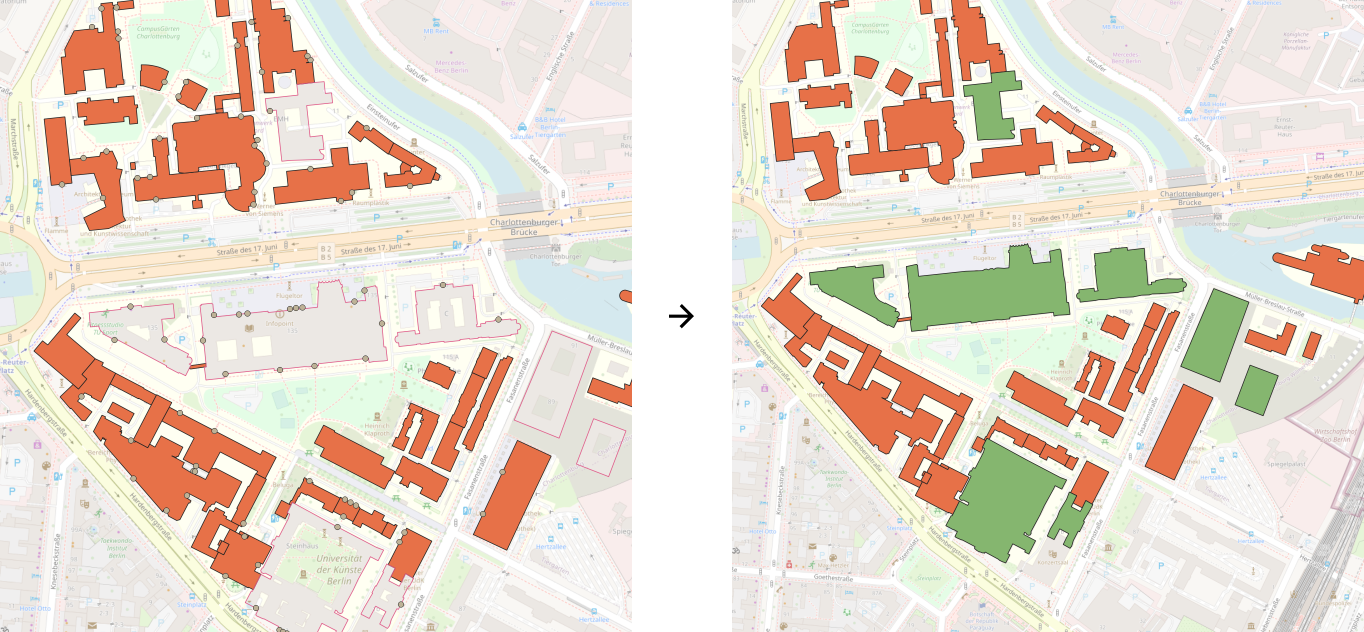
\includegraphics[width=0.65\textwidth]{images/preparing_buildings.png}\\
	\caption{Correction of TU Berlin's building data}
\end{figure}

\begin{figure}[H]
	\centering
	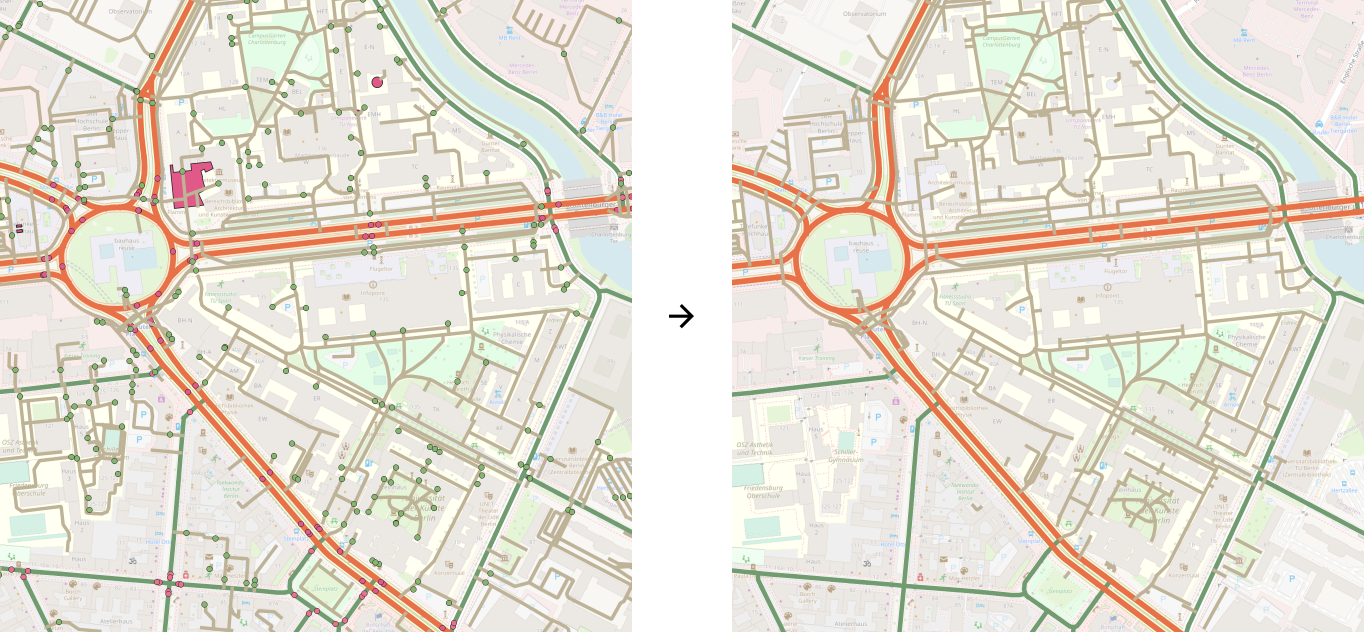
\includegraphics[width=0.65\textwidth]{images/preparing_streets.png}\\
	\caption{Correction of TU Berlin's street network data}
\end{figure}

\begin{figure}[H]
	\centering
	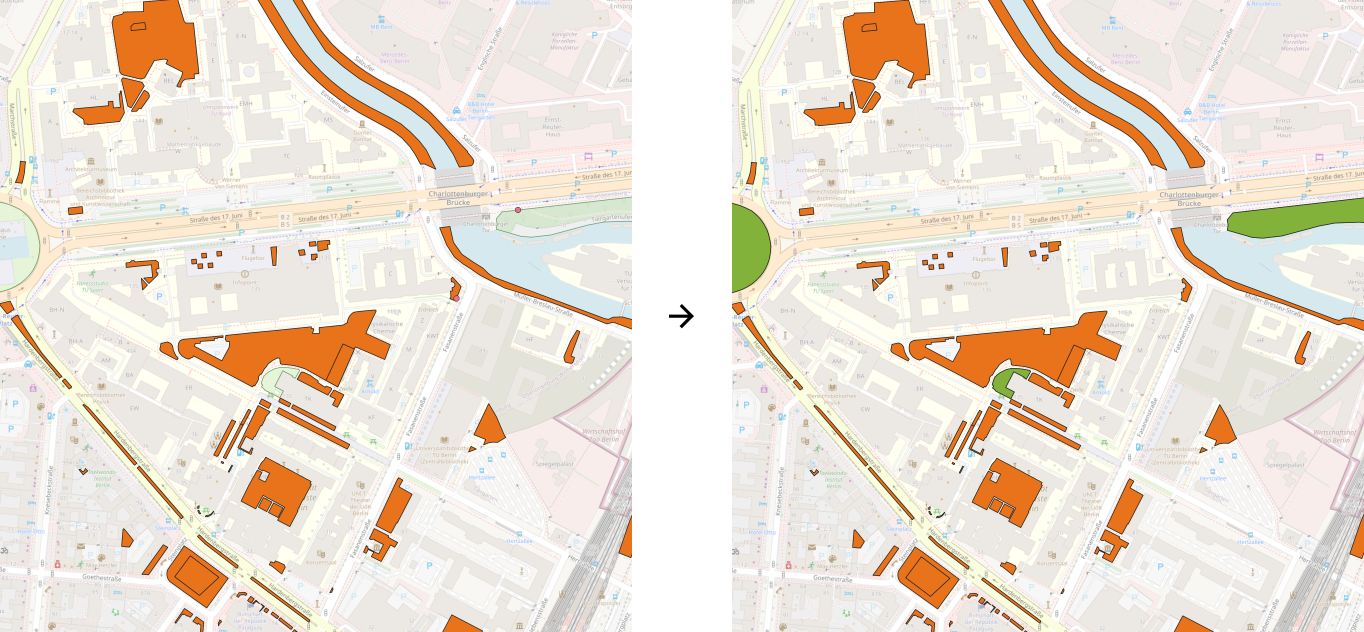
\includegraphics[width=0.65\textwidth]{images/preparing_green_areas.png}\\
	\caption{Correction of TU Berlin's green area data}
\end{figure}

\begin{figure}[H]
	\centering
	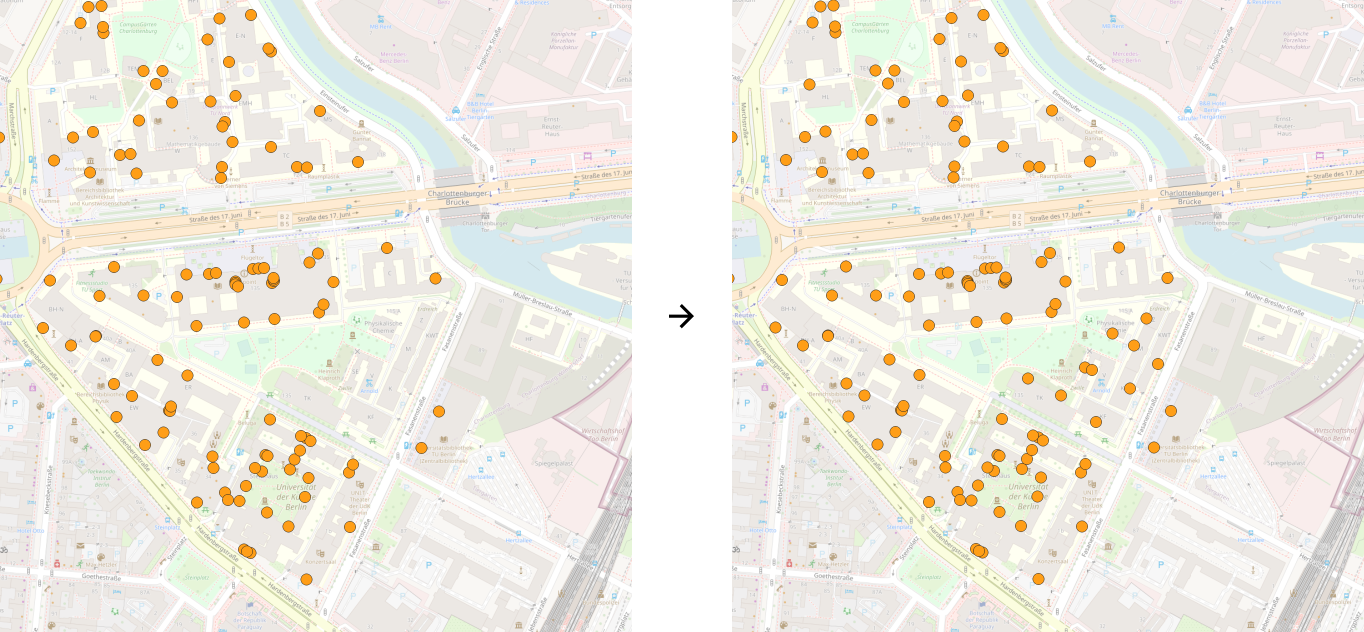
\includegraphics[width=0.65\textwidth]{images/preparing_entrances.png}\\
	\caption{Correction of TU Berlin's entrance data}
\end{figure}

The main problem that gets corrected consists of wrong geometry types in the data. Since is desirable that every dataset only contains one kind of geometry (e.g., the data for the buildings should only contain polygon outlines, the street data should only contain polylines, etc.), all wrong geometry types in a dataset are either deleted (e.g., single points in the street or building data) or reshaped to match the expected geometry type (e.g., polylines representing the outline of a building/green area are converted into polygons).

Missing entities (e.g., certain entrances to buildings) are furthermore added and information not related to the campus (mainly data from the street network) is removed.

\section{Generation of digital campus map}
This section provides a detailed overview of the procedure for generating the digital campus map in the Unity3d real-time rendering engine. It starts by describing how the already collected data is used and imported into Unity and further explains how 3d entities are created from it. The section concludes with a brief overview of the map design and the implementation details for common map gestures such as pinch-to-zoom or slide-to-move.

\subsection{Data import and conversion in Unity}
The first step in the map generation process is the import of the manually corrected OSM data from QGIS into Unity3d. This is done in geoJSON format \cite{geoJSON}, which specifies a certain JSON structure for geodata and contains all coordinate points and their relations to each other as well as additional attributes.

After import, a C\# class named GeoNode is introduced, which represents a single node in the OSM data and contains its position. Furthermore, a class for every category of entities on the campus map (buildings, green areas, streets, ...) is implemented, which contains an array of position vectors, derived from the GeoNodes, describing the respective (out)line of its entity. Lastly, methods for parsing geoJSON into their C\# object representations are created.

One main problem during the parsing process is the fact that OSM and the campus map are constructed differently: While OpenStreetMap consists of a map projected onto a sphere, the campus map is generated on a 2-dimensional plane. This results in the usage of different coordinate systems. OpenStreetMap in this case uses the WGS 84/Pseudo-Mercator system \cite{pseudo_mercator_1} \cite{pseudo_mercator_2}, which describes points on Earth as pairs of latitude and longitude. This is ideal for spherical map projection but is not suitable for a 2d plane base, where general length units (e.g., meters) are advantageous. A conversion from WGS 84/Pseudo-Mercator to 2d position vectors (x, y) in meters from the map origin is therefore chosen and integrated into the parsing process. It is further defined that x represents the longitude and y is the original latitude component of WGS 84.

The unit conversion process is based on OpenStreetMap's reference implementation of the WGS 84/Pseudo-Mercator projection \cite{mercator_projection_implementation} in C and computes the following formulas:

\[x(lon) = lon * r\]
\[y(lat) = \ln(\tan(\frac{lat}{2} + \frac{\pi}{4})) * r\]

Where the WGS 84/Pseudo-Mercator coordinates (lat, lon) in radians are converted to (x, y) in approximate meters, with r being the radius of the Earth (note that the WGS 84 coordinates are usually defined in degrees and need to be converted into radians beforehand).

The resulting coordinates are furthermore stored inside the GeoNode class as floats and are also converted into Unity's 3-dimensional Vector3 position system, where a position (x, y) is mapped to Vector3(x, 0, y). To center the campus section of TU Berlin around Unity's origin at Vector3(0, 0, 0), the central map point of campus Charlottenburg (52.5126624, 13.3231489) is subtracted from all OSM data points before conversion.

\subsection{Mesh generation for streets, green areas, water and 3d buildings}
Meshes are the building blocks for every 3-dimensional object rendered on a digital screen. They define the structure of an object and provide parameters for lighting calculations and material mapping and are generated by defining a set of attributes, the most relevant ones being:

\begin{enumerate}
	\item Vertices: Vertices are points in space, that define the corners of an object.
	\item Triangles: To generate a surface area, 3 different previously defined vertices are connected to form a triangle. A net of triangles finally determines the final shape and surface of an object. One important concept to keep in mind is the backface culling step of the render pipeline: For optimization purposes, the rendering engine decides whether surfaces created by triangles are drawn or not by using the order of vertices that define a certain triangle. Unity3d only renders triangles with a clockwise ordering of vertices when projected onto the screen. The whole process of generating a triangle net to fill a predefined surface area is called surface triangulation.
	\item Surface normals: Surface normals are vectors that are perpendicular to their related surface. They are used to differentiate between the "front" and "back" sides of their respective surface and are an important component for calculating the lighting of an object. Generally, each triangle is assigned a surface normal, which can be calculated by taking the cross product of two different edges. (Note: Unity differs from that and uses a surface normal per vertex approach. This normal can be calculated by averaging all normals of triangles containing the respective vertex. For better understanding, the normal per triangle model is nevertheless displayed in the figures.)
	\item UV coordinates: UVs are 2-dimensional coordinates that specify the texture mapping of an object. There are as many UV coordinates as vertices in a mesh. Based on the shape of an object, the UV coordinate system can be mapped differently onto the vertices.
\end{enumerate}

\begin{figure}[H]
	\centering
	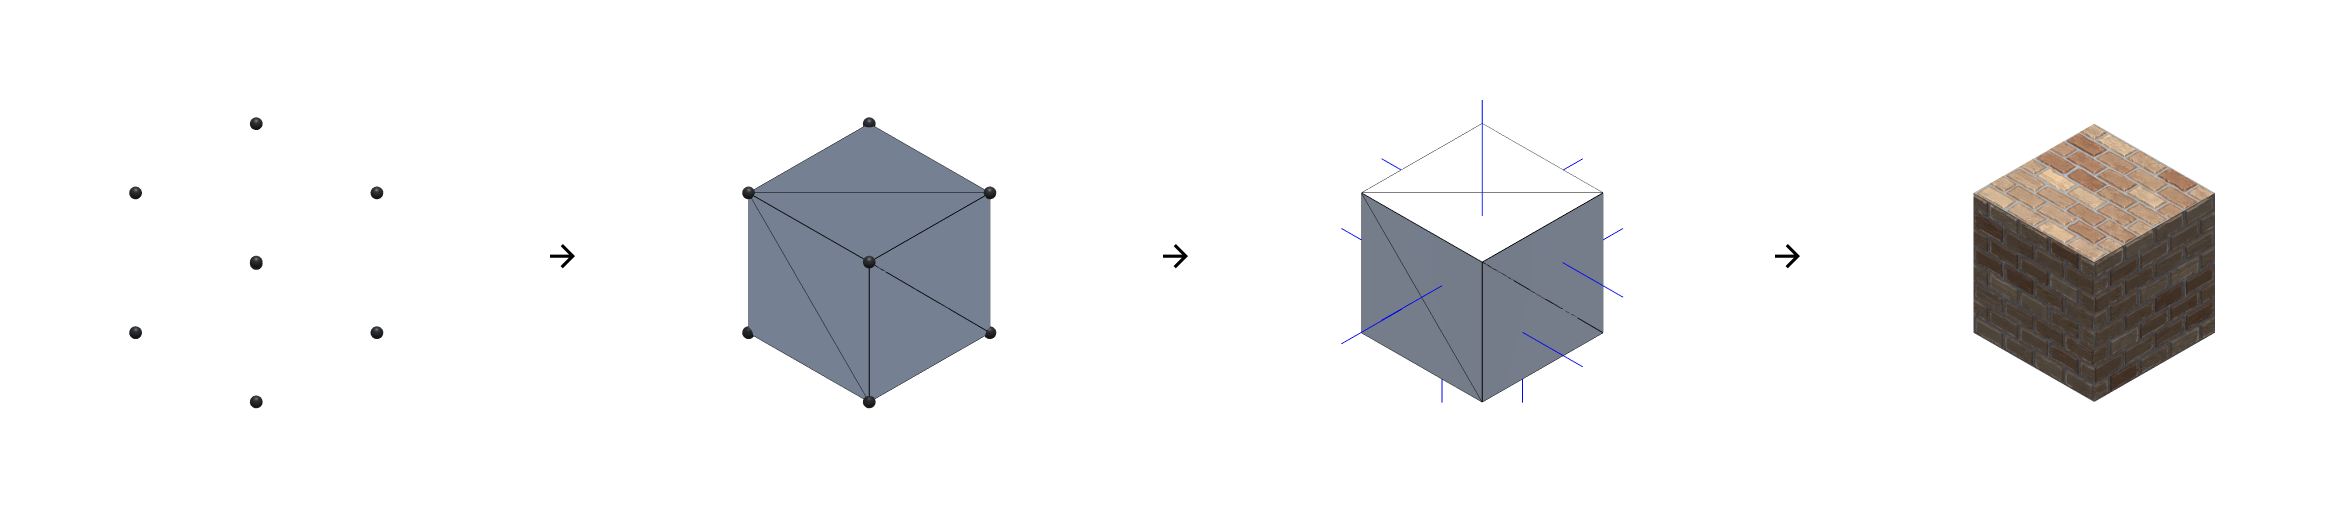
\includegraphics[width=0.8\textwidth]{images/mesh_generation_process.png}\\
	\caption{Mesh generation process for a cube}
\end{figure}

In the case of the campus map, several simplifications can be made: Surface normals can be calculated from the predefined vertices and triangles. Since the entities on the campus are only unicolored (no distortable textures are applied) the 2-dimensional UV coordinates can be chosen arbitrarily (or not at all) for every vertex. This breaks down the mesh generation process for the campus map into two separate tasks: Defining the outlining vertices of an entity from its GeoNodes and triangulating its corresponding surface.

Mesh generation for streets: To define the outline of a street, the corresponding GeoNodes, which only represent a polyline, need to be replaced by two separate polylines defining the edges of the street. The width $w$ of the street is then defined by the distance between both outlining polylines. To generate them, every GeoNode at index $i$ with coordinate $\vec{g_{i}}$ of the original polyline can be shifted with a vector $\vec{v}$, which is perpendicular to the road direction at $\vec{g_{i}}$ and the up-facing vector (in the case of Unity Vector3(0, 1, 0)). A pair of outlining points can be therefore generated for every GeoNode coordinate $\vec{g_{i}}$:

\[\vec{eRight_{i}} = (\vec{g_{i + 1}} - \vec{g_{i}}) \times (0, 1, 0) * \frac{w}{2}\]

\[\vec{eLeft_{i}} = (\vec{g_{i + 1}} - \vec{g_{i}}) \times (0, 1, 0) * - \frac{w}{2}\]

Where $\vec{eRight_{i}}$ is the point on the right polyline and $\vec{eLeft_{i}}$ is the point on the left polyline corresponding to $\vec{g_{i}}$ (when looked into the direction $\vec{g_{i + 1}} - \vec{g_{i}}$).

These vertices can be further triangulated by grouping 4 points. To fill the street surface between coordinates $\vec{g_{i}}$ and $\vec{g_{i + 1}}$, the points $A = \vec{eLeft_{i}}$, $B = \vec{eRight_{i}}$, $C = \vec{eRight_{i + 1}}$ and $D = \vec{eLeft_{i + 1}}$ are selected and two triangles $ACB$ and $ADC$ are created.

\begin{figure}[H]
	\centering
	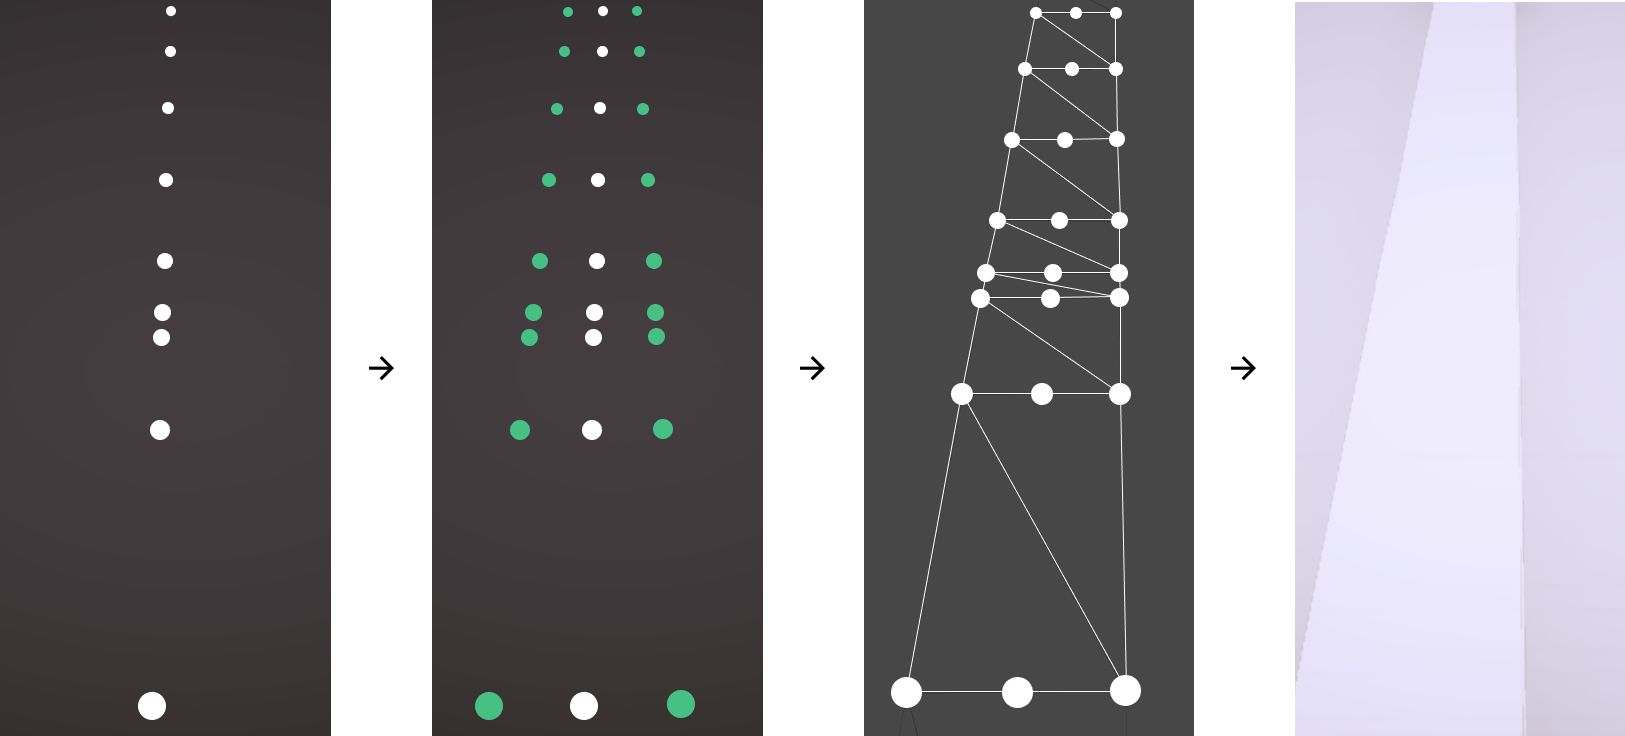
\includegraphics[width=0.8\textwidth]{images/street_mesh_generation.png}\\
	\caption{Mesh generation process for a street}
\end{figure}

Mesh generation for buildings: Buildings consist of a ceiling tile and a set of surrounding walls. To determine the outlining vertices, the predefined set of GeoNode coordinates can be extended by shifting it upwards. The amount of shift is determined by the height $h$ of the respective building. For every GeoNode coordinate $\vec{g_{i}}$, a new coordinate $\vec{c_{i}}$ is therefore created and added to the final set of building vertices:

\[\vec{c_{i}} = \vec{g_{i}} + (0, 1, 0) * h\]

The triangulation process for the resulting set of vertices can be broken down into two separate procedures for the ceiling and the walls. On the one hand, a routine similar to the street triangulation process can be applied to create the walls. A single wall is here defined by two consecutive GeoNode coordinates $\vec{g_{i}}$ and $\vec{g_{i + 1}}$ and their corresponding shifted coordinates $\vec{c_{i}}$ and $\vec{c_{i + 1}}$. The surface area between these four points is then exactly triangulated like a piece of street defined by four points (see the previous section).

On the other hand is the triangulation process for the ceiling tile. In this case, a standard algorithm for the triangulation of concave polygons can be applied. The "Triangulation by Ear Clipping" \cite{triangulation_by_ear_clipping} algorithm is used with a C\# implementation for Unity derived from \footnote{https://luminaryapps.com/blog/triangulating-3d-polygons-in-unity/index.html}. To avoid backface culling problems and for simplicity, all triangles are generated double-sided, with vertices specified in both orderings.

\begin{figure}[H]
	\centering
	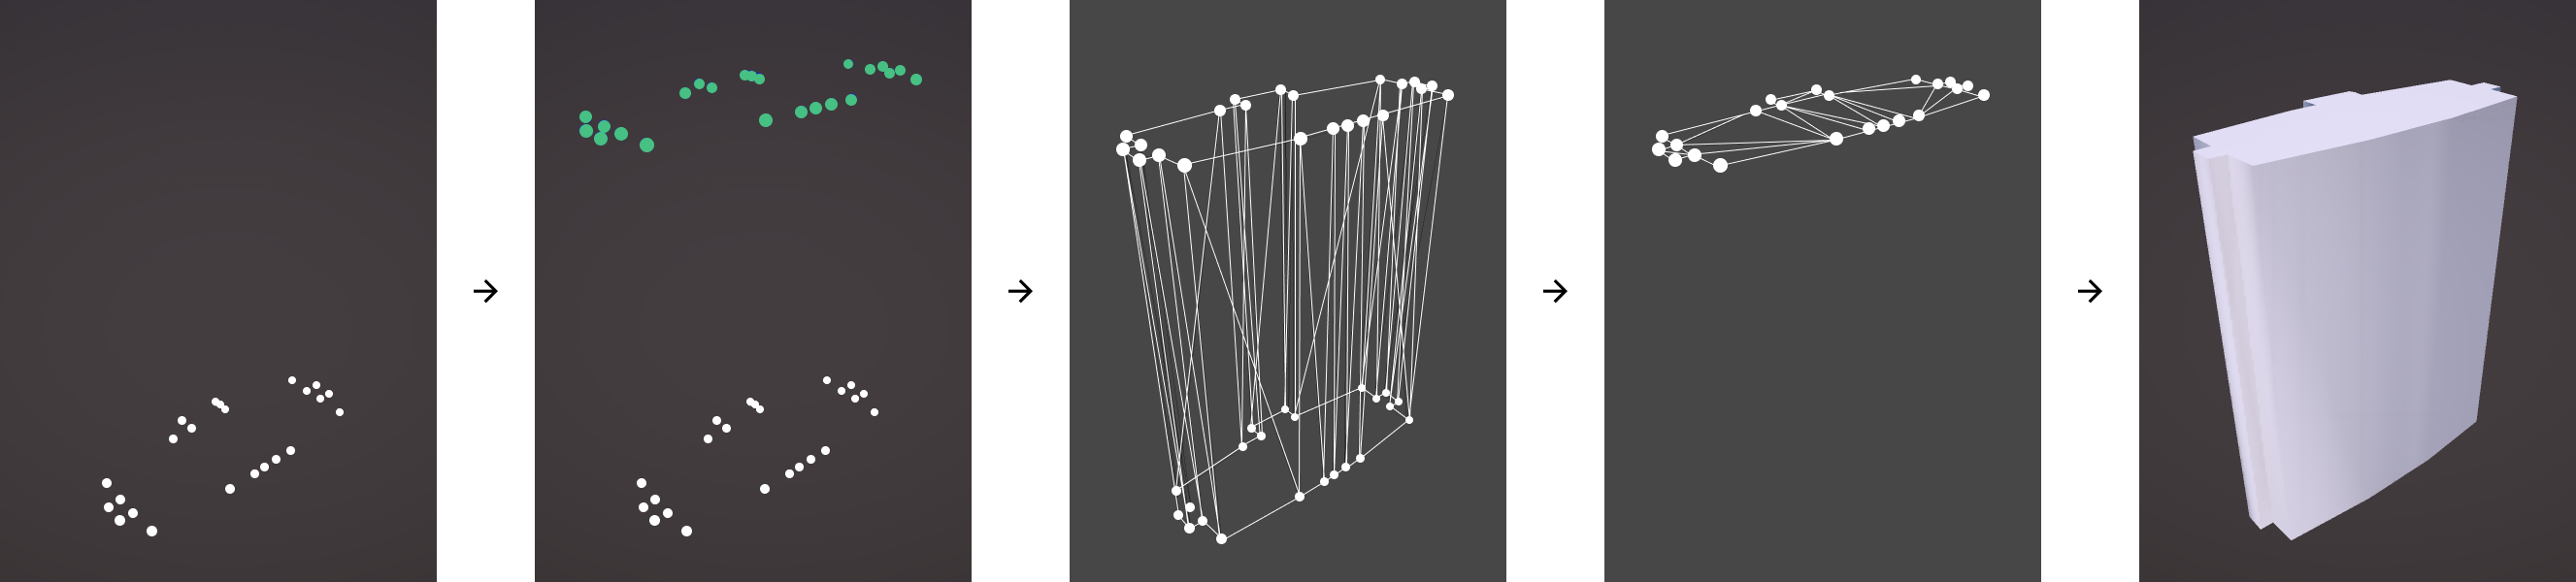
\includegraphics[width=0.8\textwidth]{images/building_mesh_generation.png}\\
	\caption{Mesh generation process for a building}
\end{figure}

Mesh generation for green areas and water: Since green areas and water both consist of flat and concave polygons, the same procedure can be used for generating both respective meshes. The outlining vertices are in this case simply the predefined GeoNode coordinates and can be triangulated in the same manner as the ceiling of a building.

\subsection{Camera setup}
One main component for the 3d rendering of the campus map is a virtual camera, that can be regarded as a viewport through which the user looks at the scene. Its transform (the set of values that determines the camera's position, rotation and scale) as well as several other parameters specifying how the scene is rendered can be manipulated to achieve a specific look of the scene.

To easily control the camera for movement, zoom and rotation, an empty and transparent object with position $\overrightarrow{p}$ is placed on the ground of the map. This focus point object is furthermore declared as the parent of the camera, which results in the fact that all camera transformations are now relative to the focus point's transform. This means, that $\overrightarrow{p}$ now serves as the camera's world origin and that the camera furthermore has two different transforms: The global transform GC, which reflects the actual position, rotation and scale of the camera in the scene and the local transform LC, which consists of the camera's position, rotation and scale relative to its parental focus point. To make it more comprehensible one can look at an example regarding the positioning of the camera: If the local position of the camera $\overrightarrow{lc}$ is at $(0, 0, 0)$ (and neither a rotation nor a scaling is anywhere applied), the camera's true global position in the scene $\overrightarrow{gc}$ is the focus point's position $\overrightarrow{p}$. In general (without rotation or scaling) $\overrightarrow{gc} = \overrightarrow{p} + \overrightarrow{lc}$, which means that the camera now "follows" the focus point object with offset $\overrightarrow{lc}$ whenever its position changes.

The camera is now locally transformed such that the focus point object always lies in the center of its viewport. In principle, this can be done arbitrarily, but to mimic the perspective of TU Berlin's official campus map \cite{campus_plan}, a setup is chosen where the camera is rotated 45 degrees down (x-axis) and $\overrightarrow{lc} = (0, z, -z), z \geq 0$ (x-axis, y-axis, z-axis). An alternative setup for top-down view (called "2d" mode inside the app) is also provided, which positions the camera directly above the focus point with a rotation of 90 degrees downwards and $\overrightarrow{lc}$ = $(0, z, 0)$. The following figure presents the setup for both cases.

\begin{figure}[H]
	\centering
	
\includegraphics[width=0.8\textwidth]{images/camera_setup.png}\\
	\caption{Camera setups for "3d" and top-down "2d" view}
\end{figure}

With this setup as a prerequisite, all map-relevant camera transformations can be defined with the parameters $\overrightarrow{p}$ (position of the focus point object), which is responsible for the camera movement, $\varphi$ (rotation of the focus point object around the y-axis), which represents the camera rotation and $z$ (parameter of the local position of the camera), which is the camera's zoom amount.

Besides the transform parameters of the camera, two other important render settings need to be considered for the campus map: On the one hand, there is the projection mode, which determines how the 3d environment is projected onto the 2d screen. Here the perspective projection is chosen since it resembles the real-world projection of the human eye and therefore creates an intuitive feeling of depth inside the scene. On the other hand, the field-of-view (FOV) value, which determines the opening angle of the camera viewport is set to 55 degrees. 

\subsection{Implementing common interaction gestures}
Touch gestures are an established way of controlling the previously defined parameters for movement, rotation and camera zoom. This section explains which gestures are chosen and how they are implemented for this thesis.

One prerequisite for a smooth and robust interaction experience is the use of animation when moving, rotating and zooming on the map. A parameter is therefore not directly set, but rather linearly interpolated over time between its current value and a desired target value. From a programming perspective, the system constantly tries to perform such an interpolation and only stops, when the actual parameter is equal to the target one. Therefore the only parameters that need to be set while interacting with the map are the target values, which are hereafter denoted as $\overrightarrow{p_{t}}$, $\varphi_{t}$ and $z_{t}$.\\

Map movement: The user can move the camera on the campus map by dragging a finger over the touchscreen. The internal evaluation of this process can be broken down into multiple steps:

\begin{enumerate}
	\item The user's finger touches the screen for the first time (touch start): The initial touch position $\overrightarrow{t_{start}}$ is detected.
	\item The user slides the finger over the touchscreen (touch moved): The current touch position $\overrightarrow{t_{cur}}$ is detected and the desired camera position is calculated as $\overrightarrow{p_{t}} = \overrightarrow{p} + (\overrightarrow{t_{start}} - \overrightarrow{t_{cur}}) * \alpha$, where $\alpha$ determines the drag speed of the campus map and is chosen as 5.
\end{enumerate}

Pinch-to-zoom: Pinching is a type of gesture where the user positions two fingers on the touchscreen and an action is triggered when the distance between both touchpoints changes. In this case, the camera should zoom in when the user brings the fingers closer together and vice versa. The following steps are necessary to implement this functionality:

\begin{enumerate}
	\item Two fingers touch the screen simultaneously for the first time (touch start): Both touch start positions are retrieved and their distance $d_{start}$ is calculated.
	\item The user moves one or more fingers (touch move): The current distance $d_{cur}$ between both fingers is calculated. The target zoom is set as $z_{t} = z_{t} + (d_{cur} - d_{start}) * s$, where $s$ is the strength of the zoom and is selected as 0,1.
\end{enumerate}

Rotation of the map: The gesture for map rotation is similar to the pinch gesture from the zoom functionality, but rather takes the rotation angle between the start- and end position of both fingers into account, instead of their distance. This can be also realized in two different steps:

\begin{enumerate}
	\item Two fingers touch the screen simultaneously for the first time (touch start): The difference between both touch positions is stored as a 2-dimensional vector $\overrightarrow{t_{sdiff}}$.
	\item  The user moves one or more fingers (touch move): The current difference of touch positions is also stored as a 2-dimensional vector $\overrightarrow{t_{cdiff}}$. The camera rotation is updated with $\varphi_{t} = \varphi + singedAngle(\overrightarrow{t_{sdiff}}, \overrightarrow{t_{cdiff}}) * \beta$, where $singleAngle(a, b)$ is a function that returns the signed angle between two 2-dimensional vectors and $\beta$ is a parameter for the rotational strength and practically set to 0,5.
\end{enumerate}

\subsection{Map design}
The last step in the campus map generation process is the elaboration of a conceptually fitting design. The requirements for such a design mainly consist of the fact that all important landmarks should be easily identifiable and explorable by the user as well as that the map should fit into the already created UI design.

For the color scheme of the map, inspiration can be taken from already established map services \cite{google_maps_website} \cite{apple_maps_website} and the real-world counterparts of the presented entities. Green areas are displayed in a green tone (HEX \#71C79D), water is displayed in blue (HEX \#90CEFF), the street network is white (HEX \#FFFFFF) and buildings are presented in a neutral grey tone (HEX \#E6E6E6).

In Unity3d, colors are applied through so-called material objects, which further also contain parameters for lighting calculations. One material is chosen per entity. The only rendering parameters, that are modified for every material, are the ones that define the light calculation model as well as shadow casting options. The latter one is turned on, which results in the fact that in contrast to \cite{google_maps_website} and \cite{apple_maps_website}, all entities on the map cast and receive shadows. The light rendering mode, on the other hand, is set to the metallic workflow mode, which offers specular reflections based on predefined "metallic" and "smoothness" values. These values are set individually for every material type.

To emphasize the 3d environment as well as to form additional reference points for orientation, tree models are placed in the green areas on the north- and south sections of the campus. Furthermore, additional building structures are manually applied onto certain buildings (e.g., Hauptgebäude and Mathematikgebäude), to more closely resemble their respective real-world shapes.

\begin{figure}[H]
	\centering
	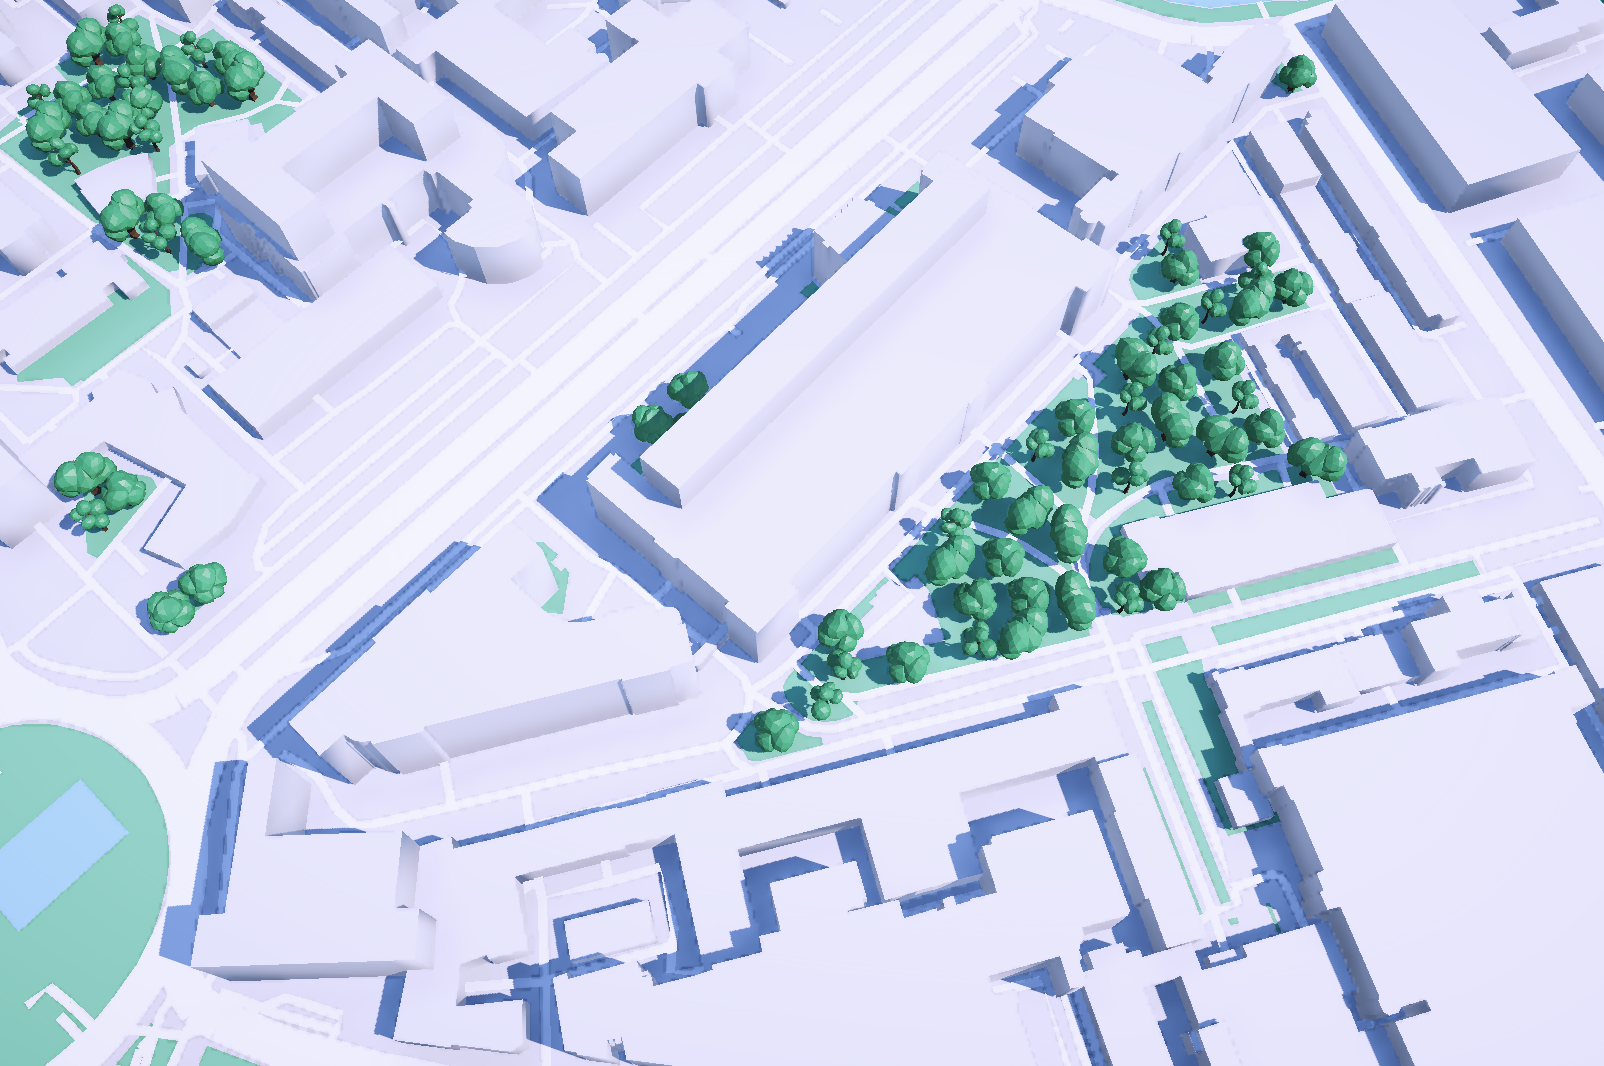
\includegraphics[width=0.8\textwidth]{images/generated_campus_map.png}\\
	\caption{Overview of the generated campus map}
\end{figure}

\section{Navigation system development}
The mobile navigation system for TU Berlin's main campus forms the most important key feature of this thesis. It provides its users the ability to navigate and localize themselves on campus Charlottenburg and utilizes the already developed campus map and its underlying street network for routing and guidance.

The following sections provide a chronological overview of the necessary steps performed to develop such a system.

\subsection{Representation of geodata for navigation}
The main building block of the navigation system is the underlying data of TU Berlin's street network and its relation to the entities on the campus. The street network is stored as a weighted graph, with individual nodes representing building entrances and control points on a path as well as edges (connections) between those nodes, describing the actual underlying street sections.

For this thesis, the graph is constructed with the so-called NavigationNode class. This class represents, when instantiated, a single node in the weighted graph, that is used in the latter routing system. It furthermore defines the connections between individual nodes as well as their relation to TU Berlin's buildings. The following table presents an overview of the attributes of the NavigationNode:

\begin{table}[!ht]
	\small
	\centering
	\begin{tabular}{|l|l|l|l|}
		\hline
		\textbf{Name}           & \textbf{Datatype}     & \textbf{Is required?}       	& \textbf{Default value} 	\\
		\hline
        id               		& int	              	& yes                          	& - 				\\
		\hline
        latitude                & double              	& yes                          	& - 				\\
		\hline
		longitude               & double              	& yes                          	& - 				\\
		\hline
		associatedBuildingId    & int              		& no                          	& null 				\\
		\hline
		connections    			& int[]              	& no                          	& [] 				\\
		\hline
	\end{tabular}
	\caption{NavigationNode class diagram}
\end{table}

\subsection{Manual generation of TU Berlin's street network} \label{sub_sec:street_network_generation}
One main problem with the street network provided by OSM is the fact that the queried data is not completely suitable for navigation. The underlying issue is that certain connections between streets are missing in the dataset, which results in problems when trying to calculate the fastest way during routing. This problem especially applies to transitions between different street types (e.g., a footway merging into a small street) and small pathways on the campus, the latter making up the biggest part of the street network used in this thesis. Another important point is the fact that there are no connections between different, sometimes completely missing, entrances of a building. This disables the possibility of including indoor segments when routing.

To improve the quality of the street network for routing, a small computer app is developed that presents the queried nodes from OSM as small dots on a map (green dots are basic nodes, red dots are nodes related to an entrance of a building). The tool provides the possibility to add additional nodes to the network as well as to create and edit connections (edges) between them (represented in blue). The manually annotated street network can be furthermore exported into a JSON file, which is stored locally in the app and deserialized into NavigationNodes during runtime. The following figure provides an overview of the manually annotated street network for navigation.

\begin{figure}[H]
	\centering
	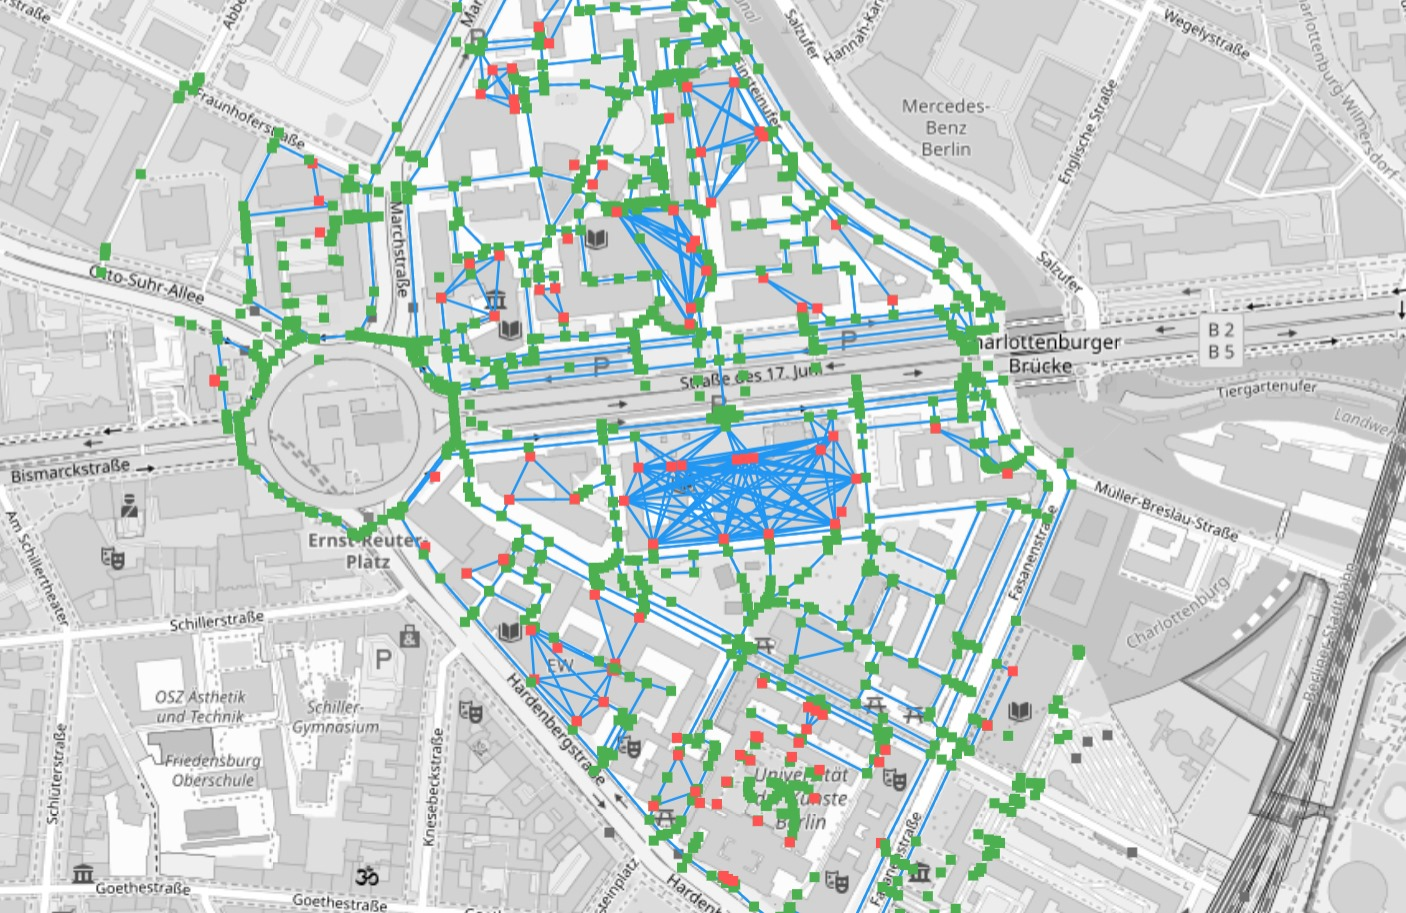
\includegraphics[width=0.8\textwidth]{images/street_network_for_navigation.jpeg}\\
	\caption{Manually annotated street network of campus Charlottenburg}
\end{figure}

\subsection{Defining weights and calculating ETA}
Weights are values assigned to edges in a graph, that represent a certain cost metric. When used in a graph for navigation purposes, they usually define how efficiently and fast a route section, defined as the edge between two nodes, can be traveled. Well-chosen weights are therefore a fundamental component for routing through a road network. This section presents the function used for determining the weight of an edge for the previously defined graph.

A weight in this thesis is defined as the (estimated) seconds needed to walk the route section defined by an edge. The following parameters are considered when choosing a weight for an edge:

\begin{itemize}
	\item Distance $d$ between both nodes that define the edge
	\item Walking speed $v$ of a human
	\item Whether traffic lights need to be passed when walking the route section
	\item Whether the edge leads through a building
	\item In case of an indoor section: Size and complexity of the respective building
\end{itemize}

The base for the weight calculation is formed by the time it takes to walk the distance of the respective route section. This can be calculated with $d / v$. Since the largest part of the users consists of younger students, the average walking speed for this age group is selected from \cite{average_walking_speed} as $v = 1,4 m/s$.

Due to the way the nodes and edges were chosen when the street network was constructed, an edge can maximally contain one pair of traffic lights on its route section. For each edge to which this applies, an additional traffic light bonus time $c_{tl}$ is added to the weight. Study \cite{traffic_light_waiting_time} portrays that $c_{tl} = 40 s$ can be chosen as an upper bound for the waiting time at a traffic light.

The last important factor that needs to be considered is the adjustment of weights for indoor route sections: Since every edge in the graph either entirely lies outdoors or completely leads through a building, the length of an indoor edge can be used as a metric to indicate the complexity and size of its respective building (longer indoor sections indicate more complex buildings, which in turn, are regarded as responsible for longer walking times). To adjust for this, the distance $d$ of the route section of an edge is multiplied by an environment factor $f$, which is either set to $f_{o} = 1$ for outdoor sections or $f_{i} = 1.05$ for indoor sections. This approximates that an indoor section takes 5\% percent longer than its equivalent outdoor section.

This results in the following equation for a weight $w$ as a function of an edge $e$ and its corresponding distance $d_{e}$:

\[
	w_{e}=\left\{
	\begin{array}{ll}
		(v * f_{o}) / d_{e} 			& \mbox{for an outdoor edge without traffic light} 	\\
		(v * f_{o}) / d_{e} + c_{tl} 	& \mbox{for an outdoor edge with traffic light} 	\\
		(v * f_{i}) / d_{e} 			& \mbox{for an indoor edge}
	\end{array}\right.
 \]

To further calculate the estimated total walking time t of a route consisting of edges 0 \ldots n, their respective weights need to be summed:

\[
	t = \sum_{i=0}^{n} w_{e_{i}}
\]

\subsection{Routing across the campus}
After defining the weighted graph for TU Berlin's street network, the fastest routes between two nodes can be calculated using a routing algorithm. For this thesis, a simple implementation of Dijkstra's algorithm for finding the shortest paths in a graph \cite{dijkstras_algorithm} is used.

\subsection{Embedding the current user location via GPS}
There are two different use case scenarios for navigation system usage: On the one hand, users can search for two different POIs on the campus and display the fastest route between them. On the other hand, a user searches for a specific destination and expects the system to directly calculate and display the route between its current location and the selected destination point. The latter scenario needs the capability to detect the user's current location, which is realized with the help of the built-in GPS module of the mobile device.

To achieve this, two different methods for resolving the GPS position are used: Firstly, to determine the starting point of the route calculation, the current position is detected with a one-shot query. After the respective route is then calculated and the live navigation functionality is initiated by the user, the GPS API is queried with a stream, continuously providing the current device position by firing a callback. This behavior can be modeled as a loop which serves as the foundation for the procedure described by \ref{fig:navigation_system}.

\section{Interactive information layer development}
The second component of the app consists of an interactive information layer that acts as a location-based service and provides the user with detailed information about TU Berlin's campus. The following sections describe the implementation details, dealing with the data model, its partition into offline and online categories and the related acquisition process from TU Berlin's and Studierendenwerk's web resources. 

\subsection{Underlying data model}
To create a foundation for the development process of the information layer, the needed data must be specified. This is done in the form of a relational database schema, consisting of all entities, their attributes and the relations between them. The fact whether a specific dataset is stored locally on the device (offline) or a web server (online) as well as the publicly available web resources, from which the data is queried are also specified in this process. The following table provides an overview of the relevant actors in this dataset:

\begin{table}[!ht]
	\small
	\centering
	\begin{tabular}{|p{3cm}|p{1cm}|p{3.5cm}|p{2cm}|p{3.5cm}|}
		\hline
		\textbf{Entity}         & \textbf{Storage type} & \textbf{Update interval}      & \textbf{Type of update} 	& \textbf{Source}					 \\
		\hline
		Building	            & offline	            & Infrastructural changes       & App update 		& TU Berlin's website		 \\
		\hline
        NavigationNode          & offline	            & Infrastructural changes       & App update 		& OpenStreetMap  			 \\
		\hline
        Canteen                 & offline              	& Infrastructural changes       & App update 	    & Studierendenwerk's website \\
		\hline
		Room               		& offline              	& Infrastructural changes       & App update 		& MOSES			      		 \\
		\hline
		Course				    & offline              	& By semester                   & App update 		& MOSES	and ISIS		     \\
		\hline
		CourseEvent	    		& offline              	& By semester                   & App update 		& MOSES			             \\
		\hline
		Event		    		& online              	& Daily                         & via REST-API 	    & TU Berlin's website		 \\
		\hline
		Meal		    		& online              	& Daily                         & via REST-API 		& Studierendenwerk's website \\
		\hline
	\end{tabular}
	\caption{Overview of information layer entities}
\end{table}

As displayed in the table, all data with low timeliness regarding the update interval is stored locally on the client device. This provides the user the possibility to access it without the need for a network connection. It nevertheless comes with the drawback that an update of the data can only take place with a complete app update, which would need to be downloaded from the respective app stores in a production use case. Online storage of the respective data with a semester-wise in-app synchronization system should be therefore taken into consideration in a real-world usage scenario. The latter point mainly applies to the course timetables ("Course" and "CourseEvent" entities), which changed by semester.

Since daily changes can occur in the meal and event datasets, both information endpoints are constantly provided via REST-API from a web server and therefore only available when a network connection can be established. To obtain a more precise overview of the individual attributes and relations of the entities, the complete database schema is provided in the following figure. Green tables represent locally stored (offline) entities.

\begin{figure}[H]
	\centering
	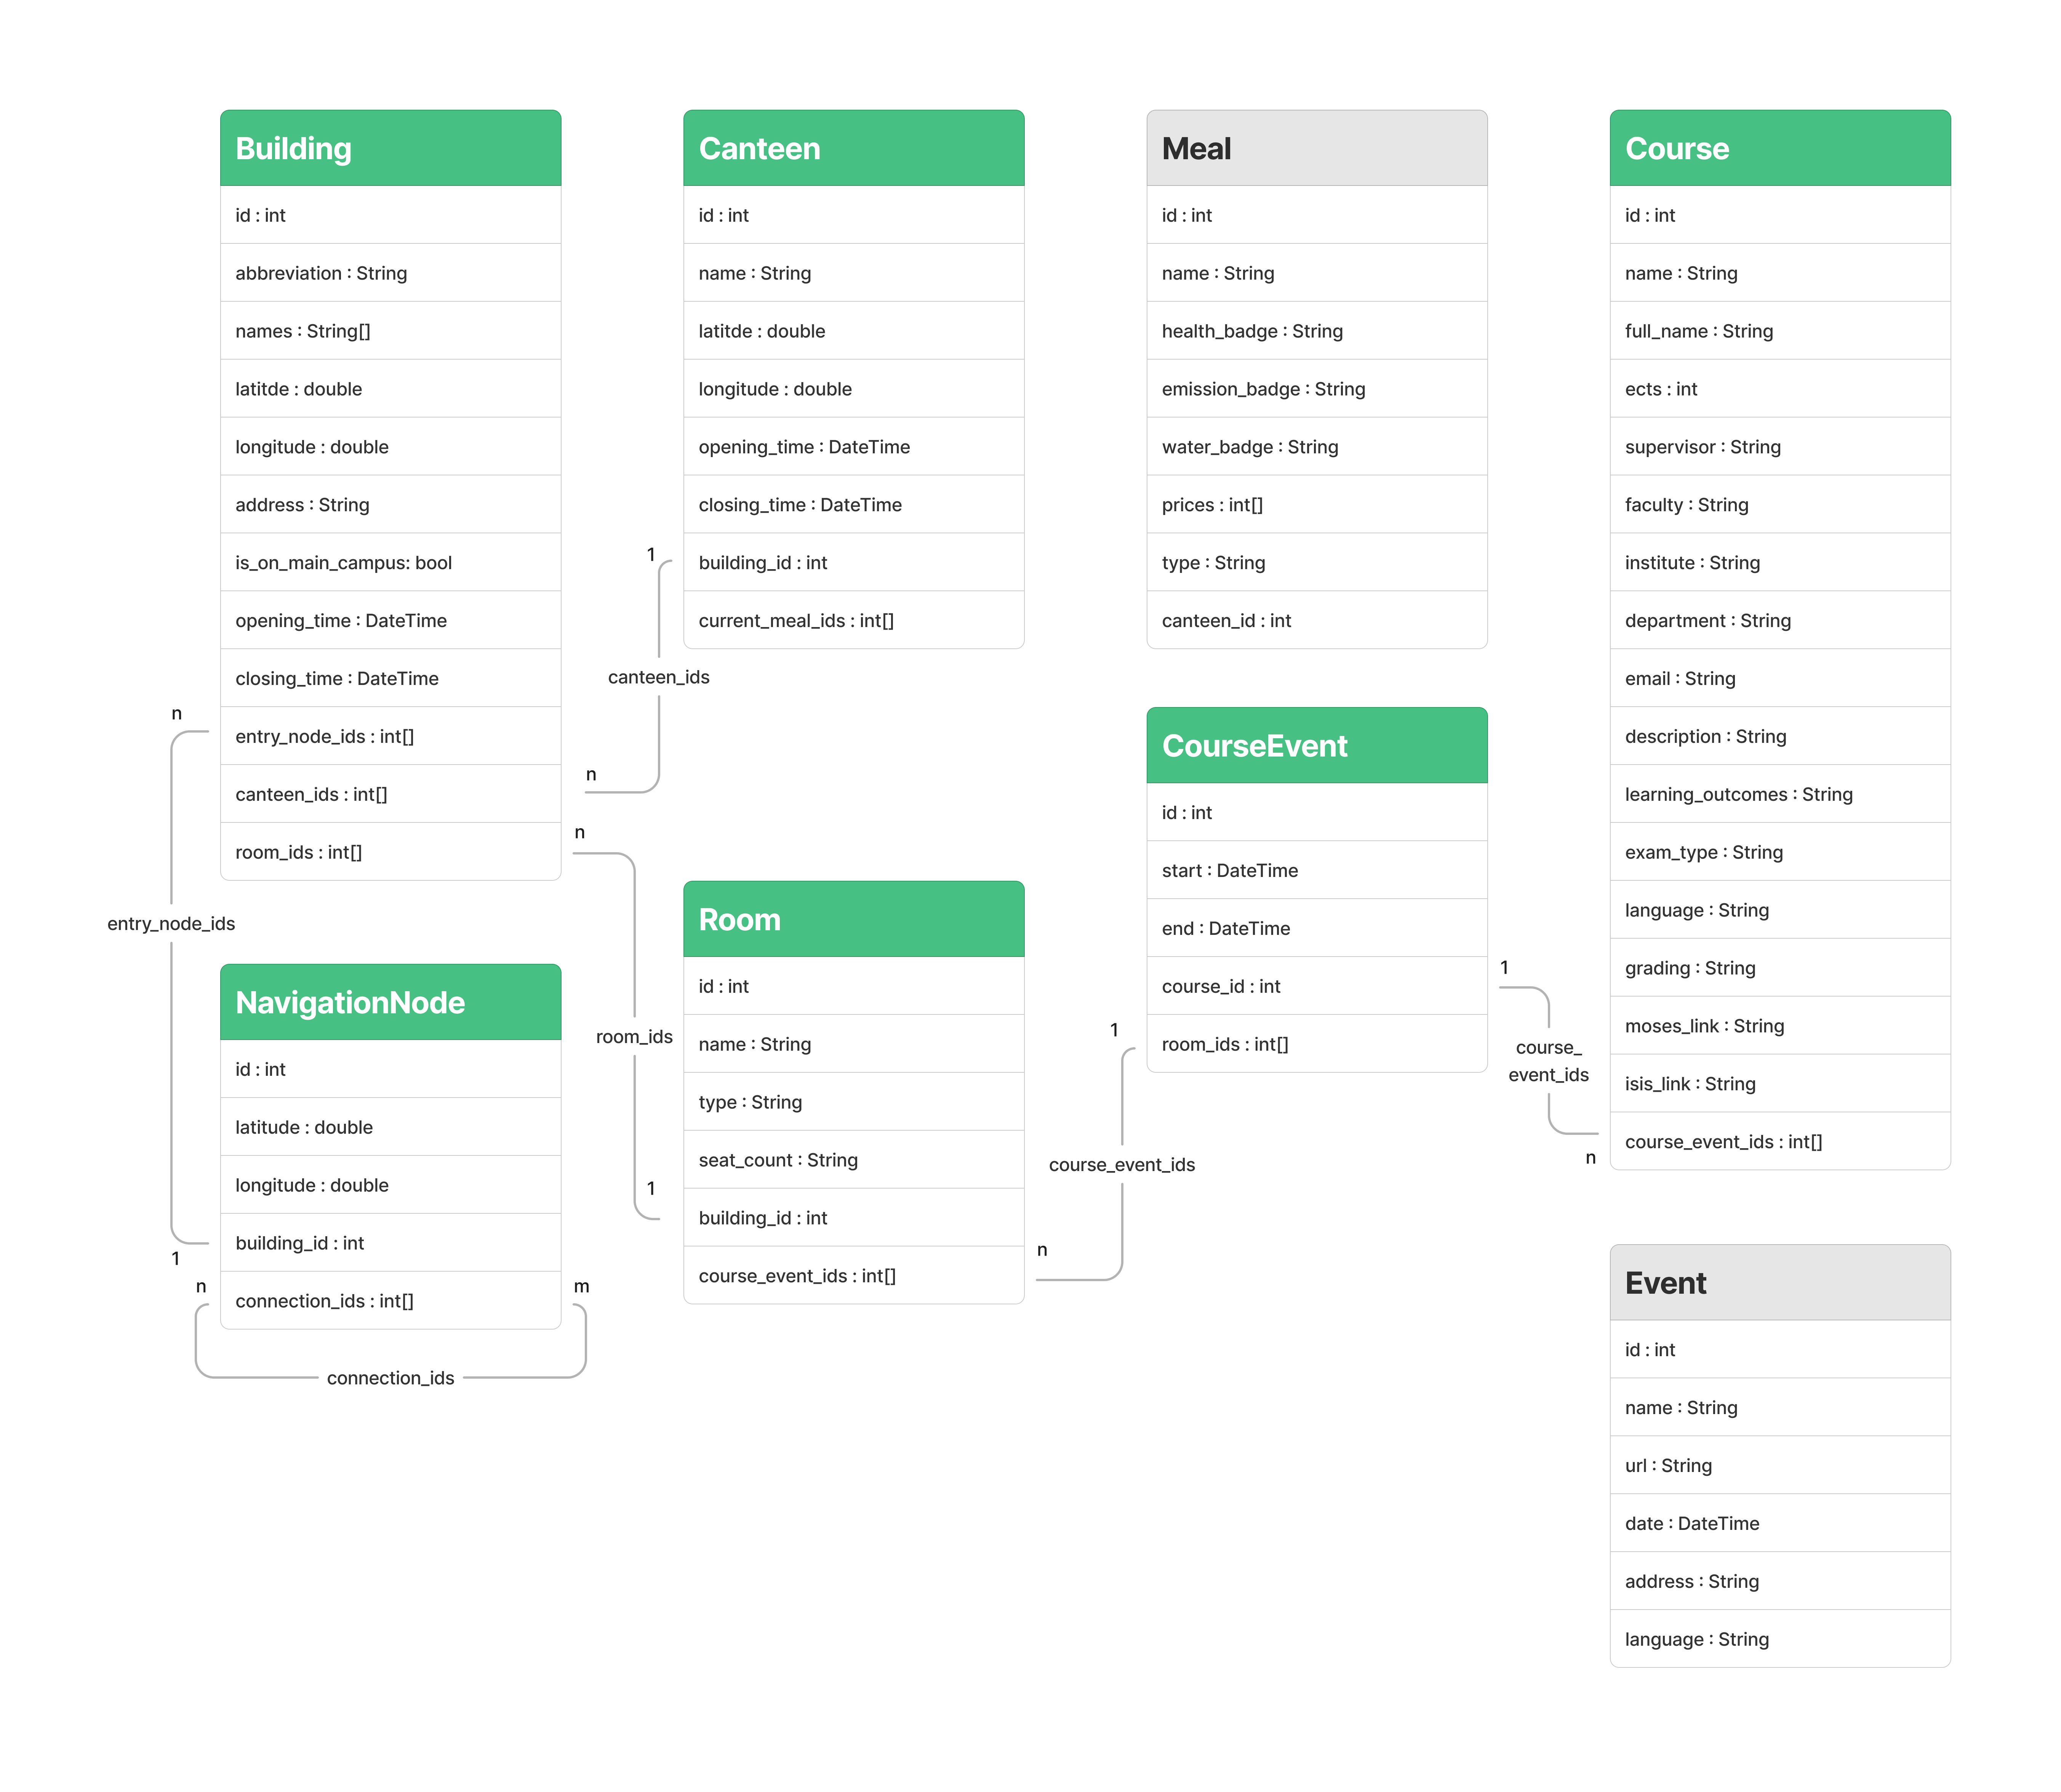
\includegraphics[width=0.95\textwidth]{images/database_schema.png}\\
	\caption{Database schema of the campus app}
	\label{fig:database_schema}
\end{figure}

\subsection{Collection of campus relevant information from the web}
The foundation for every data collection operation consists of a Python script, mainly dependent on the Beatfulsoup \footnote{https://pypi.org/project/beautifulsoup4/} package, which provides the possibility to parse HTML files and search for specific elements and their attributes in them. These scripts are then, according to the category of their dataset (offline vs. online), deployed either on a web server or used locally for data collection. This section provides a short overview of the different scripts, their deployment and the resulting data formats they produce.

NavigationNode: Data for NavigatonNodes creates the building block for the navigation system and is therefore implemented locally on the device. It is furthermore only updated when a breaking infrastructural change occurs on TU Berlin's campus. The respective acquisition script for the data is intended for manual usage and downloads the relevant information via Overpass Turbo API from OpenStreetMap. Since the downloaded data needs heavy manual annotation, the rest of the collection process is done manually with the street network tool described in the \hyperref[sub_sec:street_network_generation]{subsection for street network genetation}.

Building: Buildings are also part of TU Berlin's campus infrastructure and therefore rarely need updates. Since no central online resource contains all the data to fully describe the set of them and the amount of buildings is small compared to the size of the other datasets, the scraping process is done manually. Similar to the NavigationNode dataset, all data is locally stored on the client's device in a JSON file.

Room: Rooms are downloaded from TU Berlin's MOSES system \footnote{https://moseskonto.tu-berlin.de/moses/verzeichnis/raeume/gebaeude.html} where all rooms are provided and categorized by their respective building. The script starts by loading the provided website and then further proceeds to retrieve the room information by building from all the linked subsites. After completion, the dataset is exported in JSON format for local embedding. Room data is the third dataset connected to TU Berlin's infrastructure and therefore also only needs occasional updates.

Course and CourseEvent: The obtaining process for the course and CourseEvent datasets consists of several different steps: Firstly, all timetables containing the relevant information for the upcoming semester are downloaded from MOSES' room occupancy website \footnote{https://moseskonto.tu-berlin.de/moses/verzeichnis/veranstaltungen/raum.html?raumgruppe=31\&search=true} in CSV format. After completion, the script categorizes the different timetable data by course. This step results in the course name and its room occupancies, which are assigned to the course in the form of the CourseEvent data type. To find out all further required attributes of a course, its name is used to query the MOSES course database \footnote{https://moseskonto.tu-berlin.de/moses/modultransfersystem/bolognamodule/suchen.html}. If a fitting course is found on that page, the course's MOSES description is opened and all relevant attributes are extracted. It can be assumed that every course without a respective MOSES description is not relevant to the dataset and therefore can rejected from the dataset. To complete the data collection process, the course name is also queried against the ISIS course search \footnote{https://isis.tu-berlin.de/}, from where, if possible, a link leading to the course's ISIS page is taken. The data is finally also exported in JSON format for offline usage and is updated by semester.

Canteen: Canteens are the fourth and last entity which is usually not subject to change. This point together with the fact that TU Berlin's campus only consists of 7 different canteen leads to a manual data collection approach for this datatype. This data is also exported into a JSON file for local offline storage.

Meal: Meal plans are updated weekly (sometimes daily) on the websites of Studierendenwerk Berlin \footnote{https://www.stw.berlin/mensen/einrichtungen/technische-universit\%C3\%A4t-berlin/mensa-tu-hardenbergstra\%C3\%9Fe.html}. This means, that the data needs to be collected daily and cannot be stored locally on the client's mobile device. For the meal collection process to work, the meal table presented in \hyperref[fig:database_schema]{the database schema} is modeled into a database system running on a web server. The Python script for meal data collection is deployed as a cloud function and a CRON job, adjusted to fire daily at 00:00 o'clock, is set up to trigger the system. The cloud function then removes all the meal data stored in the database, downloads the new meals from Studierendenwerk's website and inserts them back into the online storage. A REST API connected to the database is used to provide the data to the mobile client.

Event: Events make up the second dataset that needs daily updates. They are queried from TU Berlin's online event calendar \footnote{https://www.tu.berlin/veranstaltungsdetails} and are collected in a similar way to the meal plans.

%Hier nochmal die Größe aller Daten auflisten, Anzahl Objekte, Größe der JSON-Datei, usw.

\begin{table}[!ht]
	\small
	\centering
	\begin{tabular}{|l|l|l|}
		\hline
		\textbf{Data}           & \textbf{Number of queried objects}     	& \textbf{Size on disk} 		\\
		\hline
        NavigationNode          & 1820	              					 	& 279 KB                        \\
		\hline
        Building                & 63              							& 29 KB                         \\
		\hline
		Room               		& 559              							& 53 KB                         \\
		\hline
		Course and CourseEvent 	& 1942, 31583              					& 13,9 MB                      	\\
		\hline
		Canteen    				& 7              							& 4 KB                          \\
		\hline
		Meal    				& avg. 70              						& approx. 30 KB                 \\
		\hline
		Event    				& avg. 50              						& approx. 25 KB               	\\
		\hline
	\end{tabular}
	\caption{NavigationNode class diagram}
\end{table}

The upper table presents the object count as well as the disk size of the queried data. One thing that stands out is the enormous size of the "Course and CourseEvent" data when compared to the other datasets. This aspect together with an efficient loading and processing system for this dataset, could be a possible task for future work.

\section{User interface development}
\subsection{Navigation system}
\subsection{Information layer}
\subsection{Enhancing the user experience with additional screens and features}